\documentclass{mimosis}

\usepackage{metalogo}

%%%%%%%%%%%%%%%%%%%%%%%%%%%%%%%%%%%%%%%%%%%%%%%%%%%%%%%%%%%%%%%%%%%%%%%%
% Some of my favourite personal adjustments
%%%%%%%%%%%%%%%%%%%%%%%%%%%%%%%%%%%%%%%%%%%%%%%%%%%%%%%%%%%%%%%%%%%%%%%%
%
% These are the adjustments that I consider necessary for typesetting
% a nice thesis. However, they are *not* included in the template, as
% I do not want to force you to use them.

% This ensures that I am able to typeset bold font in table while still aligning the numbers
% correctly.
\usepackage{etoolbox}

\usepackage[binary-units=true]{siunitx}
\DeclareSIUnit\px{px}

\sisetup{%
  detect-all           = true,
  detect-family        = true,
  detect-mode          = true,
  detect-shape         = true,
  detect-weight        = true,
  detect-inline-weight = math,
}

%%%%%%%%%%%%%%%%%%%%%%%%%%%%%%%%%%%%%%%%%%%%%%%%%%%%%%%%%%%%%%%%%%%%%%%%
% Hyperlinks & bookmarks
%%%%%%%%%%%%%%%%%%%%%%%%%%%%%%%%%%%%%%%%%%%%%%%%%%%%%%%%%%%%%%%%%%%%%%%%

\usepackage[%
  colorlinks = true,
  citecolor  = RoyalBlue,
  linkcolor  = RoyalBlue,
  urlcolor   = RoyalBlue,
  unicode,
  ]{hyperref}

\usepackage{bookmark}

%%%%%%%%%%%%%%%%%%%%%%%%%%%%%%%%%%%%%%%%%%%%%%%%%%%%%%%%%%%%%%%%%%%%%%%%
% Bibliography
%%%%%%%%%%%%%%%%%%%%%%%%%%%%%%%%%%%%%%%%%%%%%%%%%%%%%%%%%%%%%%%%%%%%%%%%
%
% I like the bibliography to be extremely plain, showing only a numeric
% identifier and citing everything in simple brackets. The first names,
% if present, will be initialized. DOIs and URLs will be preserved.

\usepackage[%
  autocite     = plain,
  backend      = bibtex,
  doi          = true,
  url          = true,
  giveninits   = true,
  hyperref     = true,
  maxbibnames  = 99,
  maxcitenames = 99,
  sortcites    = true,
  style        = numeric,
  ]{biblatex}

%%%%%%%%%%%%%%%%%%%%%%%%%%%%%%%%%%%%%%%%%%%%%%%%%%%%%%%%%%%%%%%%%%%%%%%%
% Tables
%%%%%%%%%%%%%%%%%%%%%%%%%%%%%%%%%%%%%%%%%%%%%%%%%%%%%%%%%%%%%%%%%%%%%%%%
%
% DEFINED BY RUI - NOT IN THE TEMPLATE

\usepackage{tabulary}

%\input{bibliography-mimosis}
\addbibresource{Thesis.bib}

%%%%%%%%%%%%%%%%%%%%%%%%%%%%%%%%%%%%%%%%%%%%%%%%%%%%%%%%%%%%%%%%%%%%%%%%
% Fonts
%%%%%%%%%%%%%%%%%%%%%%%%%%%%%%%%%%%%%%%%%%%%%%%%%%%%%%%%%%%%%%%%%%%%%%%%

\ifxetexorluatex
  \setmainfont{Minion Pro}
\else
  \usepackage[lf]{ebgaramond}
  \usepackage[oldstyle,scale=0.7]{sourcecodepro}
  \singlespacing
\fi

\renewcommand{\th}{\textsuperscript{\textup{th}}\xspace}

\newacronym[description={Principal component analysis}]{PCA}{PCA}{principal component analysis}
\newacronym                                            {SNF}{SNF}{Smith normal form}
\newacronym[description={Topological data analysis}]   {TDA}{TDA}{topological data analysis}

\newglossaryentry{LaTeX}{%
  name        = {\LaTeX},
  description = {A document preparation system},
  sort        = {LaTeX},
}

\newglossaryentry{Real numbers}{%
  name        = {$\real$},
  description = {The set of real numbers},
  sort        = {Real numbers},
}

\makeindex
\makeglossaries

%%%%%%%%%%%%%%%%%%%%%%%%%%%%%%%%%%%%%%%%%%%%%%%%%%%%%%%%%%%%%%%%%%%%%%%%
% Incipit
%%%%%%%%%%%%%%%%%%%%%%%%%%%%%%%%%%%%%%%%%%%%%%%%%%%%%%%%%%%%%%%%%%%%%%%%

\title{Usage of network emulators for the benefit of teaching and learning}
%\subtitle{A minimal, modern \LaTeX{} package for typesetting your thesis}
\author{Rui Carvalho}

\begin{document}

\frontmatter
  % !TEX root = ../Thesis.tex
\begin{titlepage}
  \vspace*{5cm}
  \makeatletter
  \begin{center}
    \begin{Huge}
      \@title
    \end{Huge}\\[0.1cm]
    %
    % \begin{Large}
    %   \@subtitle
    % \end{Large}\\
    %
    % \emph{by}\\
    \@author
    %
    \vfill
    A document submitted in partial fulfillment
    of the requirements for the degree of\\
    \emph{Technical Report}\\
    at\\
    \textsc{Miskatonic University}
  \end{center}
  \makeatother
\end{titlepage}

\newpage
\null
\thispagestyle{empty}
\newpage

  % !TEX root = ../Thesis.tex
% !TEX spellcheck = en-US

\begin{center}
  \textsc{Abstract}
\end{center}
%
\noindent
%
Scientific documents often use \LaTeX{} for typesetting. While numerous
packages and templates exist, it makes sense to create a new one. Just
because.


  \tableofcontents

\mainmatter

  % !TEX root = ../Thesis.tex
% !TEX spellcheck = en-US

\chapter{Introduction}
\label{ch:introduction}

This first chapter introduces the challenge of using virtual, fully software-based alternatives to computer network labs in education, with special emphasis on the undergraduate and graduate levels of the university. % TODO should university by capitalized here?
It also proposes the definitions that, though not universal or unique, help precise differences between those software solutions, namely two main concepts: simulation and emulation. % TODO universal NOR unique?
Together with the last point, this chapter also explains the reason why this thesis is centered, starting from its title, in ``emulators'' more than on ``simulators''.
Finally, it gives a very brief overview of the work that has already been done in the field of computer networks simulators and emulators, and, orthogonally, in the replacement of laboratories with (physical) hosts and routers/switches in schools and universities by simulated or emulated (virtual) solutions.

% end of intro

\section{Motivation and problem statement}
\label{sec:motivation}

On most education institutions, computer networks teaching has used physical laboratories, making it possible for students to exercise experimentally the knowledge acquired in the theoretical component of subjects whose program envisions going beyond skills strictly related to programming exercises---i.e. that involves contact with real networks and concrete equipment.
The existence of those laboratories is, even today, standard practice in many institutions of higher education. FCT/NOVA, which is not an exception, has a room with routers and switches for performing those practical exercises.

Despite its virtues, starting with responding to a pedagogical need in the teaching of Engineering for applying the learned theory and getting ``hands on'' experience, this method raises problems such as the cost and fast obsolescence~\cite{automaticnetconfiggns} of equipments, the demand for individual presence on the laboratory (at least for manipulating physical links and network interfaces) for exercise elaboration, the possible damage due to misuse~\cite{teachinginovation} or simple wear-and-tear, the time and effort to prepare and setup for given exercises, which may even ``destroy'' the setup for other exercises, etc. % TODO avoid repeating "exercise" so much here

Aiming to address these problems, not exclusive from further or higher education, extending to vocational education on high schools and ``\emph{politécnicos}'', and even ``courses'' of the industry itself, of which Cisco's CCNA~\cite{ccna} is a good example, or even distance learning, tools for emulating and/or simulating networks and networking equipment have been developed for years. % TODO replace "extending". o "vocational education" veio do linguee
These tools can, through the usage of several techniques, surpass some (if not all) of the aforementioned disadvantages.

\subsection{The lab on a laptop}
\label{subsec:replacingthelab}

% end of subsec replacingthelab

\subsection{Emulation, simulation (and virtualization)}
\label{subsec:emulsimvirt}

% end of subsec emulsimvirt

% end of section motivation

\section{Related work}
\label{sec:relatedwork}

% PROBABLY SOME SUBSECTIONS GO HERE

% \subsection{The lab on a laptop}
% \label{subsec:replacingthelab}

% % end of subsec replacingthelab

% \subsection{Emulation, simulation (and virtualization)}
% \label{subsec:emulsimvirt}

% % end of subsec emulsimvirt

% end of section gns3performance

\begin{figure}
  \centering
  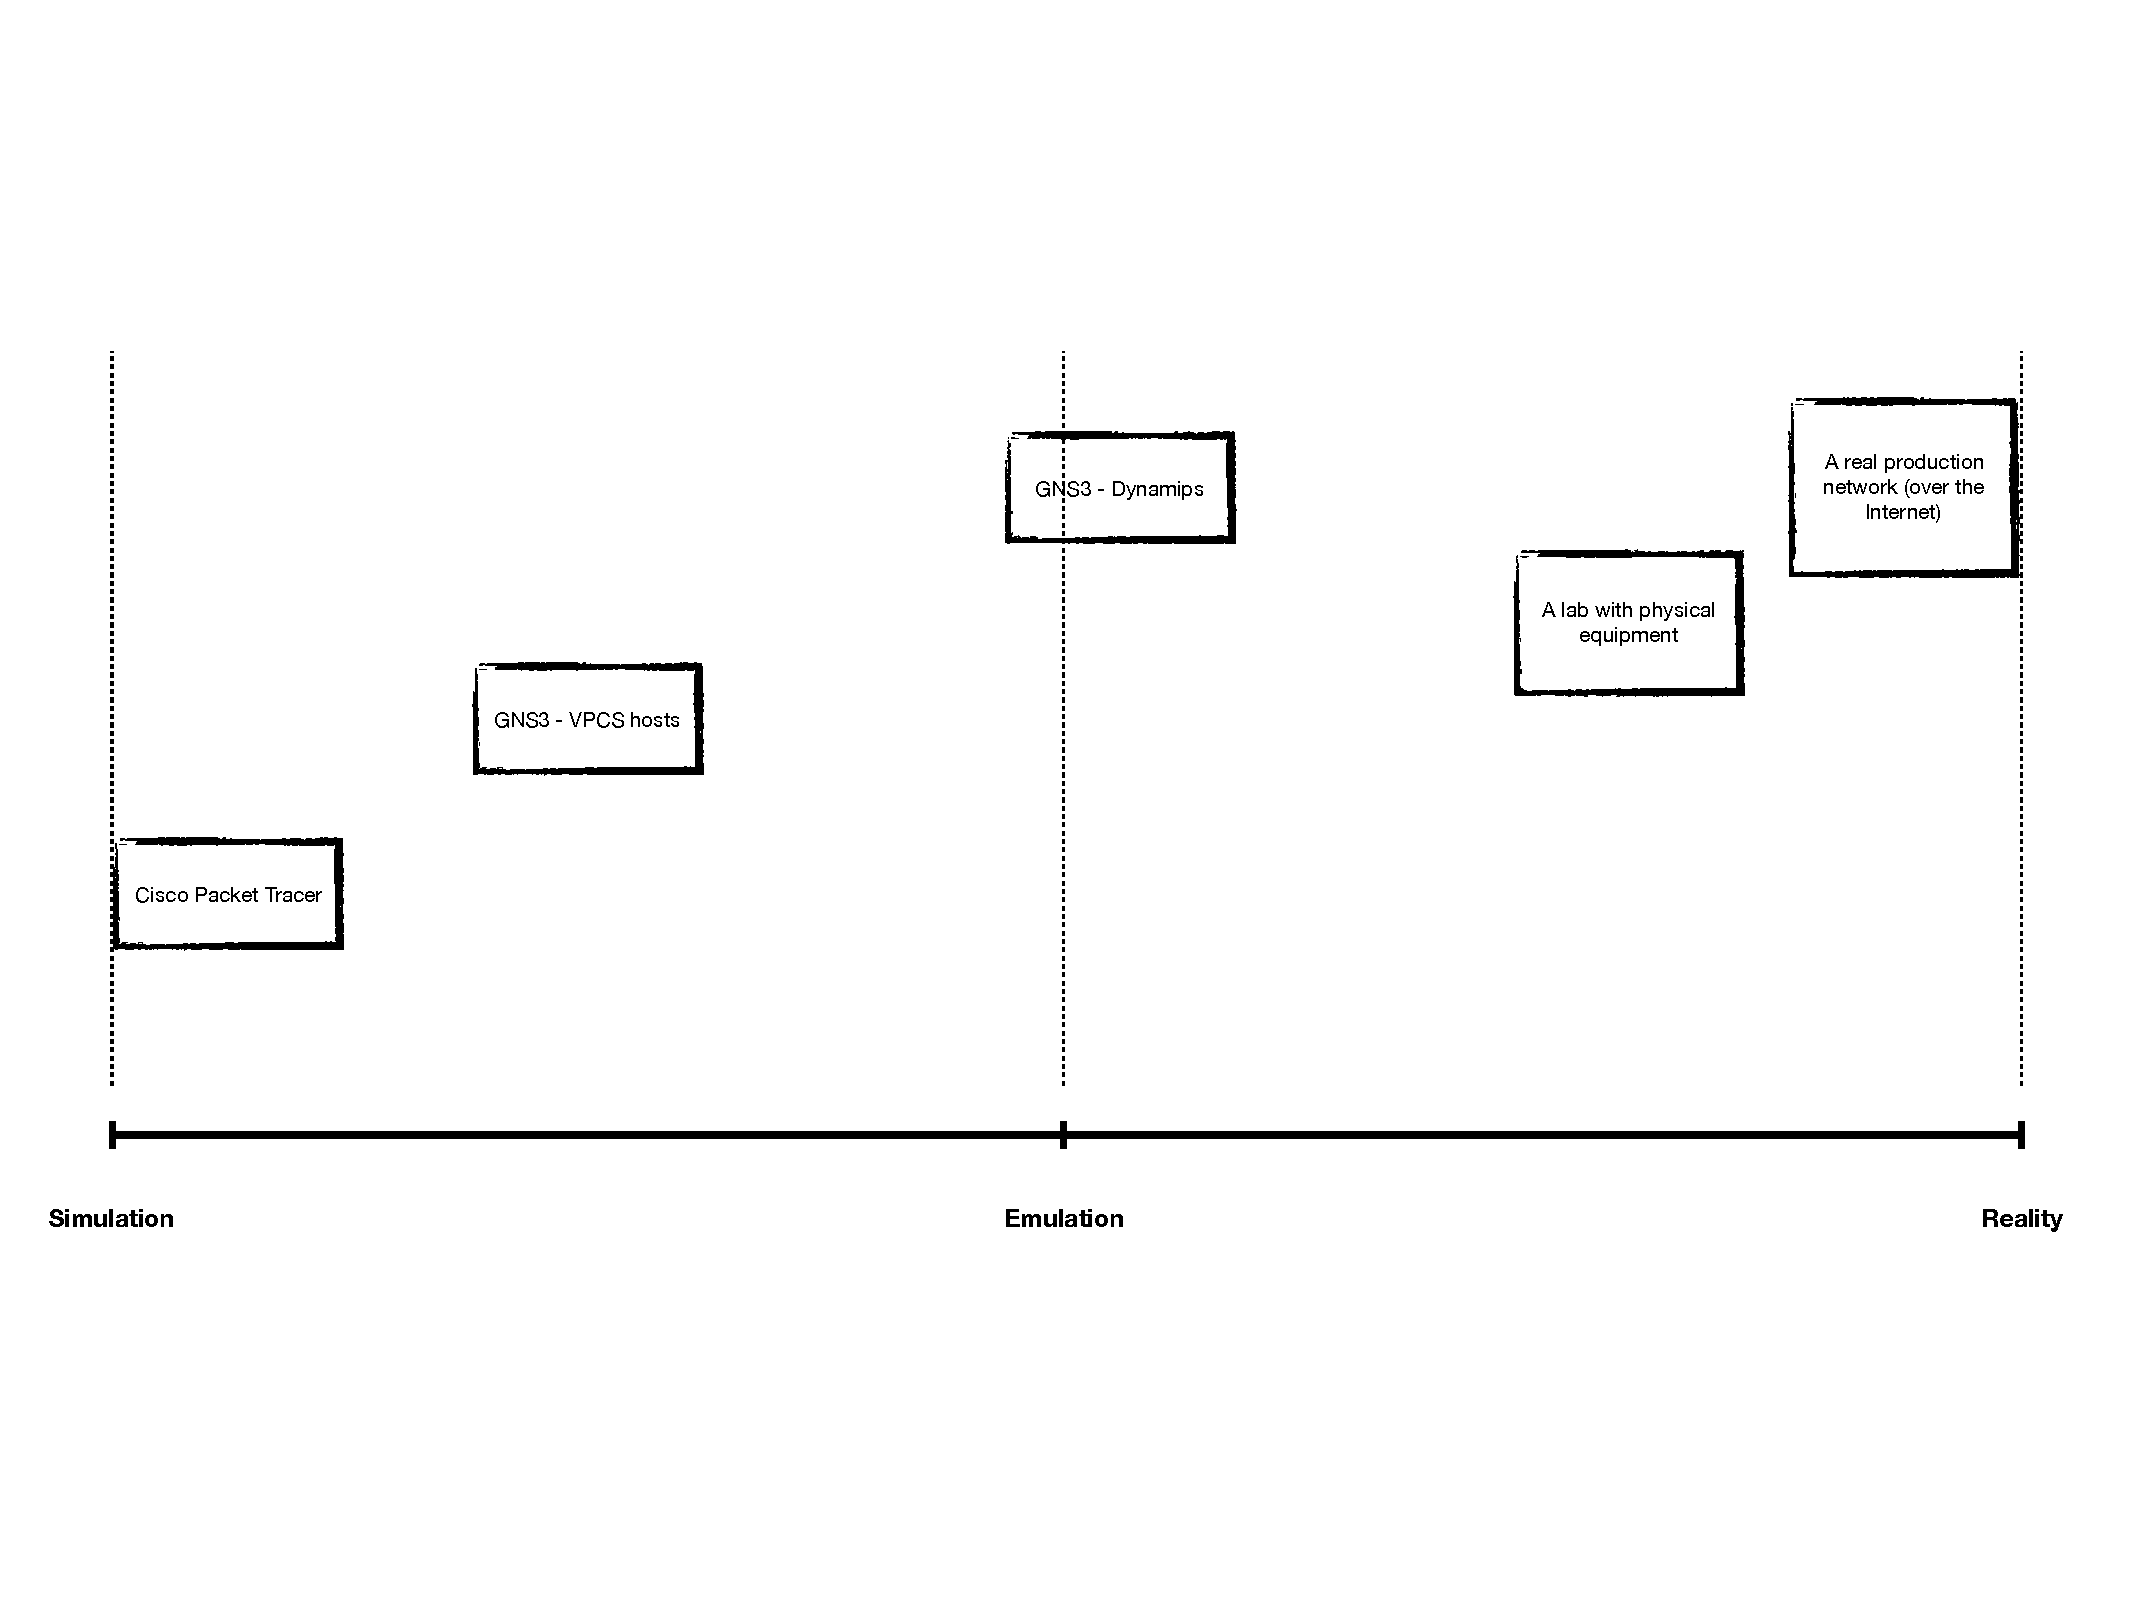
\includegraphics[width=0.8\textwidth]{emulationvsreality}
  \caption{Simulation vs emulation vs reality}
  \label{fig:emulationvsreality}
\end{figure}

% \section{The first section of this intro}
% Here we can comment on the super-interesting aspects of the diagram depicted in figure~\ref{fig:emulationvsreality}.

\section{Structure of the thesis}
\label{sec:structure}

% end of section structure

% end of chapter

  % !TEX root = ../Thesis.tex
% !TEX spellcheck = en-US

\chapter{GNS3}
\label{ch:gns3}

GNS3, whose original title was ``Graphical Network Simulator-3,'' is a software project, comprising several distinct components and, despite the ``simulator'' in its name, \emph{as a whole} falls under the category that, in this thesis, is called \emph{emulator}.
By ``as a whole,'' it is meant that, as shall be seen later, although some of its components, like the Dynamips program, are emulators in a strict sense---i.e. serve to run real machine code on a different (than its native one) hardware architecture---, it differentiates itself on a high-level perspective from a simulator which is a program designed to execute a mathematical model, processing modeled events as internal data-structures with a collection of preset algorithms that somehow mimic (a part of) the reality.

% end of intro

\section{GNS3's purpose and \emph{raison d'être}}
\label{sec:gns3why}

The GNS3 project was created by Jeremy Grossmann at the University.
It was built with a main goal: allowing students of Cisco certifcations to be able to test network topologies and practice their skills with the same software stack that is used in real Cisco devices and the hosts connected to them---from the operating system, up until application--level network utilities---, without having to use the expensive official solutions for that, or having to fall back on the limited graphical simulators like Cisco's Packet Tracer.

Despite still having a strong relation with training for Cisco CCNA and related certifications, the magnitude of the project, part of which comes from an inherent extensibility, has made it suitable for a myriad of use-cases, of which testing and configuring topologies in the context of the modern \emph{DevOps}-driven infrastructure setup and implementation is a good example.
But also potential applications that are still relatively unexplored.
Such is the case of its usage in academic teaching and learning, the goal of of this work.

% end of section gns3why

\section{Building blocks. The programs ``inside'' GNS3}
\label{sec:gns3buildingblocks}

Here's a cool table that I made where I have put systematic information about the repositories and stuff like that.

\begin{table}
  \centering
  \small
  \begin{tabulary}{0.8\textwidth}{lLL}
    \toprule
      \textbf{Part}  & \textbf{Role}                                                       & \textbf{Source code repository}\\
    \midrule
      GNS3 GUI       & A desktop application that runs on a graphical OS                   & \scriptsize\url{https://github.com/GNS3/gns3-gui}\\
      Dynamips       & A MIPS emulator, used by the \emph{backend} to run (old) IOS images & \scriptsize\url{https://github.com/GNS3/dynamips}\\
    \bottomrule
  \end{tabulary}
  \caption{%
    Intrinsic parts of GNS3, constituting separate and independent codebases
  }
  \label{tab:gns3components}
\end{table}


\subsection{GNS3 GUI}
\label{subsec:gns3gui}

Interaction between the end-user and GNS3 is usually---though, as will be clear, not necessarily---made in a graphical environment.
A GNS3 project, called a \emph{topology}, is constantly opened on one single window (per running instance of the application) and is graphically represented in the main section of the window.

\subsection{Dynamips}
\label{subsec:gns3dynamips}

The Dynamips emulator is a standalone \emph{free} program, written in C, that, normally, comes distributed together with the whole GNS3 package.
It is an emulator of a MIPS processor and was the original--single way to run the software of the Cisco nodes of the topologies created with GNS3.

% end of section gns3buildingblocks

\section{General architecture}
\label{sec:gns3architecture}

% end of section gns3architecture

\section{GNS3 in action}
\label{sec:gns3inaction}

% end of section gns3inaction

\section{Performance and resources considerations}
\label{sec:gns3performance}

% end of section gns3performance

% end of chapter

  %\include{Sources/Related}
  %\include{Sources/Workplan}

% This ensures that the subsequent sections are being included as root
% items in the bookmark structure of your PDF reader.
\bookmarksetup{startatroot}
\backmatter

  \begingroup
    \let\clearpage\relax
    \glsaddall
    \printglossary[type=\acronymtype]
    \newpage
    \printglossary
  \endgroup

  \printindex
  \printbibliography

\end{document}
